\section{Umgang mit Daten}
\begin{description}
\item[Ohne DataBinding:] Programmierer alles selbst, viel zu umständlich, mühsam und fehleranfällig
\item[Mit DataBinding: ] Lesen/Setzen von Properties erfolgt automatisch.
\begin{itemize}
    \item UI via DataContext und Data Binding-Ausdruck verdrahtet
    \item Zustandsänderung an das gebundene Property wird automatisch synchronisiert (TwoWay-Binding)
    \item kein \code{Name} Attribut mehr nötig
\end{itemize}
\end{description}

\paragraph{Markup Extensions}
\begin{description}
\item[\code{x:Type [Datentyp]}] Liefert angegebene Klasse
\item[\code{x:Static [Pfade]}] Bindet eine Konstante, statische Property, Feld oder Enum
\item[\code{x:Null}] Null Wert
\item[\code{StaticResource [Name]}] Statische Bindung an Ressource
\item[\code{DynamicResource [Name]}] Dynamische Bindung an Ressource
\item[\code{Binding ...}] Data Binding Ausdruck
\item[\code{RelativeSource ... }] Setzt die Data Binding Source auf eine relevanten Bezug im Logical Tree
\item[\code{TemplateBinding ...}] Bindet Wert an Eigenschaft des mittels Template dargestellten Controls
\item[\code{x:Reference ...}] Abk. für \verb+{Binding Elementname=...}+
\end{description}

\subsection{Überblick Syntax}
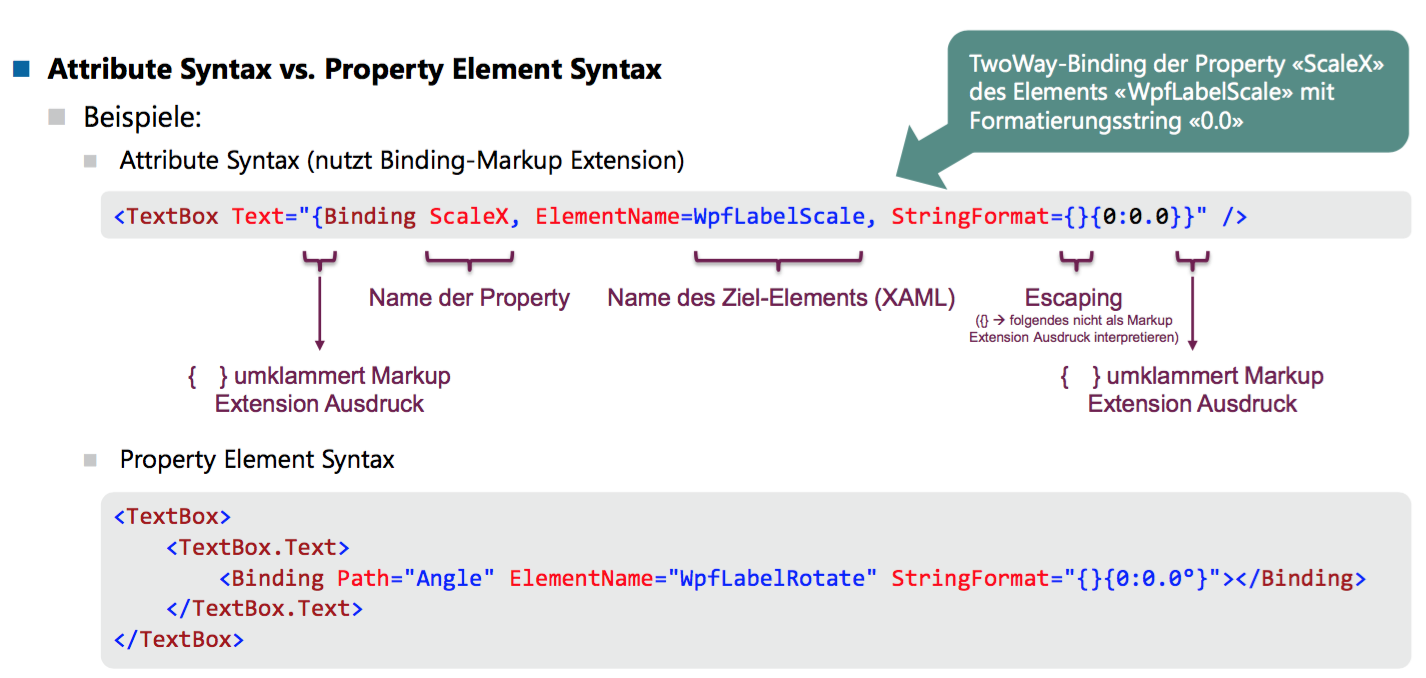
\includegraphics[scale=0.4, angle=90]{DataBinding.png}


\subsection{MultiBinding}
MltiBinding muss mit der Property Syntax gemacht werden:
\begin{lstlisting}[language=xml]
<TextBlock>
  <TextBlock.Text>
    <MultiBinding StringFormat="{}{0} -- Now only {1:0.00}!">
      <Binding Path="Description"/>
      <Binding Path="Price"/>
    </MultiBinding>
  </TextBlock.Text>
</TextBlock> 
\end{lstlisting}


\subsection{Überblick DataBinding}
\paragraph{Voraussetzungen} 
DataContext des Fensters muss auf das Modell gesetzt sein. Die gebundene Model-Klasse muss INotifyPropertyChanged implementieren falls man Änderungnotifikationen haben will.
\paragraph{Binding Base}
\begin{description}
\item[\code{Delay}] Verzögerung in Millisekunden zwischen DataBinding Operation
\item[\code{FallbackValue}] Standardwert, falls Data Binding nicht funktioniert
\item[\code{StringFormat}] Formatierungsangabe für die Umwandlung des Quellwertes in einen String  (für Beispiel siehe MultiBinding oben)
\item[\code{TargetNullValue}] Standardwert, falls Quellwert == null
\end{description}
\paragraph{Binding}
\begin{description}
    \item[\code{BindsDirectlyToSource}] Soll Angabe der Path-Property relativ zum aktuellen Datenprovider (\verb+true+) oder relativ zum Datenkontext (\verb+false+) ausgewertet werden (Nur selten sinnvoll)
    \item[\code{Converter}] Converter der beim Binding benutzt werden soll
    \item[\code{ConverterCulture}] Länderspezifische Einstellungen (\verb+CultureInfo+), welche beim Konvertieren benutzt werden soll
    \item[\code{ConverterParameter}] Zusätzlicher Parameterwert, der dem Converter übergeben werden soll
    \item[\code{ElementName}] Name des XAML-Elements auf welches gebunden werden soll
    \item[\code{Mode}] Richtung des DataBinding (OneTime, OneWay, TwoWay, OneWayToSource)
    \begin{description}
    \item[OneTime:] Eimalig (beim ersten Zugriff)
    \item[OneWay:] Lesend
    \item[TwoWay:] Lesend und Schreibend
    \item[OneWayToSource:] Schreibend
    \end{description}
    \item[\code{Path}] Pfad zur Datenquelle, Objektpfadsyntax
    \item[\code{XPath}] XPath Ausdruck zum Zugriff auf eine XML Datenquelle
    \item[\code{RelativeSource}] Setzt Datenquelle auf Objekt relative zum Ort des aktuellen Elements
    \item[\code{Source}] Setzt Datenquelle
    \item[\code{UpdateSourceTrigger}] Zeitpunkt zu welchem DataBinding getriggert wird
    \begin{description}
        \item[Default] Nutzt festgelegte Trigger der Ziel Property
        \item[Explicit] Nur beim expliziten Aufruf von \verb+UpdateSource()+
        \item[LostFocus] Fokusverlust des Elements
        \item[PropertyChanged] Bei jeder änderung des Inhalts
    \end{description}
\end{description}

\subsection{DataContext, Source, RelativeSource}
Die Datenquelle ist standartmässig nicht gesetzt, muss also explizit gesetzt werden. 

\paragraph{DataContext}
ganzes Fenster via View Model direkt im Code-Behind:
\begin{lstlisting}[language=java]
public partial class MainWindow : Window {
  public MainWindow() {
    InitializeComponent();
    var vm = new PersonViewModel();
    DataContext = vm; 
} }
\end{lstlisting}

\begin{lstlisting}[language=xml]
<TextBlock Text="{Binding FirstName}" />
\end{lstlisting}

ganzes Fenster via ViewModel als Propery im Code-Behind:
\begin{lstlisting}[language=java]
public partial class MainWindow : Window {
  public PersonViewModel MyViewModel { get; set; } // als Property zur Verfügung gestellt
  public MainWindow() {
    InitializeComponent();
    MyViewModel = new PersonViewModel();
    DataContext = MyViewModel;        
} }
\end{lstlisting}

\begin{lstlisting}[language=xml]
<TextBlock Text="{Binding FirstName}" />
\end{lstlisting}

Ganzes Fenster im Code-Behind, aber mit Fenster selbst als View-Model (this)
\begin{lstlisting}[language=java]
public partial class MainWindow : Window { 
  public PersonViewModel MyViewModel { get; set; }
  public MainWindow() {
    InitializeComponent(); 
    MyViewModel = new PersonViewModel();
    DataContext = this;
} }
\end{lstlisting}

\begin{lstlisting}[language=xml]
<TextBlock Text="{Binding MyViewModel.FirstName}" />
\end{lstlisting}

Ganzes Fenster direkt im Code-Behind aber mit Fenster als Liste
\begin{lstlisting}[language=sharpc]
PersonList = new ObservableCollection<PersonViewModel>(list); 
DataContext = this; 
\end{lstlisting}
\begin{lstlisting}[language=xml]
<ListBox ItemsSource="{Binding PersonList}">...</ListBox>
\end{lstlisting}

Direkt im XAML
\begin{lstlisting}[language=xml]
<Window.DataContext>
  <local:PersonViewModel />
</Window.DataContext>
\end{lstlisting}

\paragraph{Source} Ermöglicht die Angabe der Datenquelle direkt im DataBinding Ausdruck. Dieses Property kann auf Ressourcen (Static/Dynamic) oder statische (Static) binden.
\begin{lstlisting}[language=xml]
<!-- falls wir eine eigene String-Table haben und diese als Ressource verfügbar ist --> 
<Label Content="{Binding NameLabelCaption, Source={StaticResource Strings}}" /> 

<!-- falls wir die Beschriftung direkt als String-Ressource definiert haben--> 
<Label Content="{Binding Source={StaticResource MyNameLabelCaption}}" /> 

<!-- zum Vergleich: die bereits bekannte Kurzform mittels StaticResource-Markup Extension --> 
<Label Content="{StaticResource MyNameLabelCaption}" Margin="0,0,0.4,0" /> 
\end{lstlisting}

\paragraph{RelativeSource} 
\begin{itemize}
    \item Ermöglicht die Angabe einer relativen Datenquelle im Visual Tree
    \item Eigene Markup Extension dafür: \code{{RelativeSource ....}}
\end{itemize}

\begin{description}
    \item[\code{FindAncestor}] Sucht übergeordnetes Element des Typs (AncestorType) 
    \item[\code{PreviousData}] Bindet auf das vorhergehende Element (nutzbar z.B. in Collections Delta-Vergleiche) 
    \item[\code{Self}] Bindet auf das Element selbst 
    \item[\code{TemplatedParent}] Bindet auf Element, für welches Control Template gilt (nur innerhalb Template sinnvoll) 
    \item[\code{AncestorLevel}] Gibt Vorgänger-Position an, 1 = erster gefundener Vorgänger, 2 = zweiter, etc. 
    \item[\code{AncestorType}] Typ des zu suchenden Vorgänger-Elements 
\end{description}

\begin{lstlisting}[language=xml]
<Label Content="{Binding RelativeSource={RelativeSource FindAncestor, AncestorType=Window}, Path=Title}" />
\end{lstlisting}


\paragraph{Path} 
\begin{description}
    \item[Path Standard-Property] \code{{Binding Firstname} == {Binding Path=Firstname}}
    \item[\code{{Binding}}] Bindet direkt an Datenquelle selbst (als Ganzes)
    \item[\code{{Binding Address.Street}}] Bindet an Property Street der Property Address der Datenquelle
    \item[\code{{Binding Groups[0].Name}}] Bindet an Name des ersten Objekts in Groups-Auflistung der Datenquelle
\end{description}
\paragraph{Mode}
\begin{description}
    \item[OneTime:] Einmalig (bei erstem Zugriff) 
    \item[OneWay:] Lesend
    \item[TwoWay:] Lesend und schreibend 
    \item[OneWayToSource:] Schreibend 
\end{description}

\paragraph{Binding an anderes Element (Binding Path)}
Mit diesem Code kann man den Inhalt von, z.B. einem TextBlock, an die Eingaben in, z.B. einer Textbox, binden. In diesem Beispiel machen wir dies gleich noch durch ein MultiBinding, der Binding-Ausdruck an sich ist aber allgemeingültig.
\begin{lstlisting}
<TextBox Name="FirstName" />
<TextBox Name="LastName" />
<TextBlock>
    <!-- Anzeige: "FirstName LastName" -->
    <MultiBinding StringFormat="{}{0} {1}">
        <!-- Binden an FirstName.Text -->
        <Binding ElementName="FirstName" Path="Text" />
        <Binding ElementName="LastName" Path="Text" />
    </MultiBinding>
</TextBlock>
\end{lstlisting}

\paragraph{StringFormat}
Umwandeln eines Wertes in einen String (zur Anzeige). Funktioniert auch mit MultiBinding.
\begin{lstlisting}[language=xml]
<TextBox Text="{Binding ScaleX, ElementName=WpfLabelScale, StringFormat={}{0:0.0}}" /> 
\end{lstlisting}

\subsection{Converter}
\paragraph{IValueConverter} Ein Interface welches alle Converter implementieren müssen
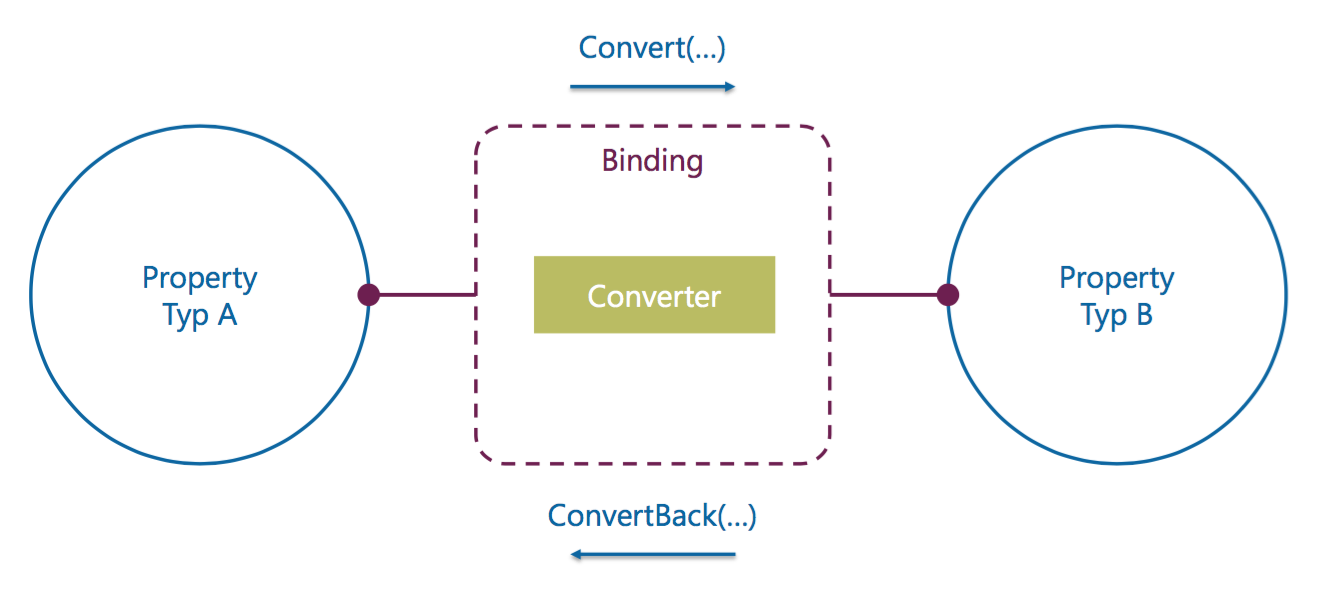
\includegraphics[scale=0.25]{IValueConverter.png}

Es ist auch möglich, nur eine der Methoden zu überschreiben und die andere mit NotImplementedException auszustatten, wenn man es selber nicht verwendet \\
\\
Konvertiert bool oder Nullable in Visibility und zurück
\begin{lstlisting}
public sealed class BooleanToVisibilityConverter: IValueConverter
{
    // value = bool oder nullable, targetType = Visibility
    public object Convert(object value, Type targetType, object parameter, CultureInfo culture)
    {
        return value is bool && (bool)value == true ? Visibility.Visible : Visibility.Collapsed;
    }
    // value = Visibility value, targetType = bool
    public object ConvertBack(object value, Type targetType, object parameter, CultureInfo culture)
    {
        return value as Visibility? == Visibility.Visible
    }
}
\end{lstlisting}
\paragraph{IMultiValueConverter} Konvertiert die Werte der einzelnen Binding-Quellen eines MultiBindings in einen einzelnen Zielwert und umgekehrt. Das Interface dass alle MultiConverter implementieren müssen. Anwendungsbeispiel: Basieren auf einzelnen Farbkomponenten eine Instanz der Color Klasse berechnen resp. die Color Klasse in deren Einzelteile zerlegen.
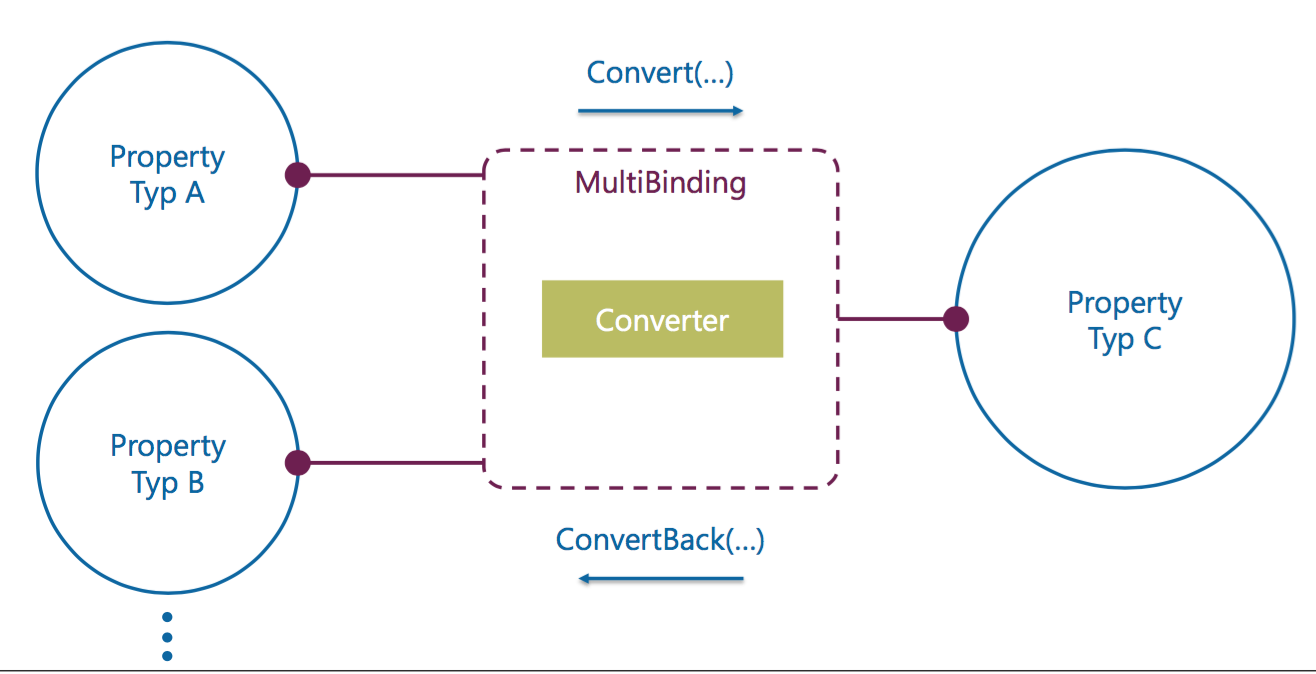
\includegraphics[scale=0.25]{IMultiValueConverter.png}
\begin{lstlisting}
public class RgbToColorConverter: IMultiValueConverter
{
    // values = Werte der binding quelle  
    // Type = Rückgabetyp     parameter = optionaler Parameter um konvertierung genauer zu steuern
    public object Convert(object[] values, Type targetType, object parameter, CultureInfo culture)
    {
        if (values == null)
            return DependencyProperties.Unsetvalue;
        if(values.Length != 3)
            throw new NotSupportedException("3 Values needed)";
        var r = (byte)System.Convert.ToInt32(values[0]);
        var g = (byte)System.Convert.ToInt32(values[1]);
        var b = (byte)System.Convert.ToInt32(values[2]);
        return Color.FromRgb(r,g,b);
    }
    public object[] ConvertBack(object value, Type[] targetType, object parameter, CultureInfo culture)
    {
        if(value == DependencyProperty.UnsetValue)
            return null;
        if(value is Color)
        {
            var color = (Color) value;
            var colors = new object[] {color.R, color.G, color.B};
            return colors;
        }
        return null;
    }
}
\end{lstlisting}
\paragraph{Value Converter anwenden} Um einen Converter anwenden zu können wird eine Instanz benötigt. Instanziierung:
\begin{lstlisting}[language=xml]
<Window.Resources>
    <local:RgbToColorConverter x:Key="MyRgbToColorConverter" />
    <local:BestContrastingColorConverter x:Key="MyBestContrastingColorConverter" />
</Window.Resources>
\end{lstlisting}
Danach kann man den Converter wie gewohnt nutzen:
\begin{lstlisting}
<SolidColorBrush>
    <SolidColorBrush.Color>
        <MultiBinding Converter="{StaticResource MyRgbToColorConverter}">
            <Binding ElementName="ColorR" Path="Value"></Binding>
            <Binding ElementName="ColorG" Path="Value"></Binding>
            <Binding ElementName="ColorB" Path="Value"></Binding>
        </MultiBinding>
    </SolidColorBrush.Color>
</SolidColorBrush>
<SolidColorBrush Color="{Binding Path=Content, ElementName=ColorLabel,
    Converter={StaticResource MyBestContrastingColorConverter}, Mode=OneWay}" />
\end{lstlisting}
Wenn man eigene Value Converters implementiert wird der XAML Code kürzer und man hat eine Entkopplung von Wert und dessen Darstellungseigenschaften. Aber es ist aufwändig und teilweise nicht trivial.



\paragraph{Bindung auf eigene Objekte} 

% Die sogenannten \textbf{DependencyProperties} ermöglichen ein Two-Way Binding und funktionieren mit Key-Value Dictionaries.Sie sind spezialisiert für die Vewendung in einem UI und somit nicht geeignet für Business Objects.
% \begin{lstlisting}
% public int MyProperty
% {
%   get {return (int(GetValue(MyPropertyPropert); }
%   set { SetValue(MyPropertyProperty, value); }
% }
% public static readonly DependencyProperty MyPropertyProperty = 
%     DependencyPropery.Register("MyProperty", 
%             typeof(int), 
%             typeoof(ownerclass), 
%             new PropertyMetadata(0));
% \end{lstlisting}


Mit dem \verb+INotifyPropertyChanged+ Interface können Properties einer Klasse überwacht werden. Das Interface schreibt das Event \verb+PropertyChanged+ vor, das implementiert werden muss. Der Event Handler übermittelt den Namen der geänderten Property.
\begin{lstlisting}
public class PersonV2 : INotifyPropertyChanged {
  public event PropertyChangedEventHandler PropertyChanged;
  // use the name of the calling property if none given:
  private bool SetProperty<T>(ref T field, T value,  [CallerMemberName] string name = null){
    if (Equals(field, value)) { return false; } // basic check for equality...
    field = value;
    PropertyChanged?.Invoke(this, new PropertyChangedEventArgs(name)); 
    return true; 
  } 
  private string _firstName;
  public string FirstName { 
    get { return _firstName; }
    set { SetProperty(ref _firstName, value, nameof(FirstName));
}
 // repeat pattern for other properties... } 
}
\end{lstlisting}
Dies kann auch mit einer Basisklasse gelöst werden, welche die Benachrichtigung implementiert.
\begin{lstlisting}
public abstract class BindableBase: INotifyPropertyChanged
{
    public event PropertyChangedEventHandler PropertyChanged;
    protected bool SetProperty<T>(ref T field, T value, string name = null)
    {
        if(Equals(field,value))
            return false;
        field=value;
        OnPropertyChanged(name);
        return true;
    }
    protected void OnPropertyChanged(string name = null)
    {
        PropertyChanged?.Invoke(this, new PropertyChangedEventArgs(name));
    }
}
public class Person: BindableBase
{
    private string _firstName;
    public string FirstName;
    {
        get { return _firstName; }
        set { SetProperty(ref _firstName, value, nameof(FirstName)); }
    }
}
\end{lstlisting}
\paragraph{Berechnete Properties} Hat man zusammengesetzte Properties, wie zum Beispiel ein FullName, welcher sich aus dem First- und den LastName zusammensetzen, so muss man bei einer Änderung eines Teiles, auch das berechnete Property updates. Das geschieht mit einem Param-Array.
\begin{lstlisting}
protected bool SetProperty<T>(ref T storage, T value, string name, params string[] otherNames)
{
    if(Equals(storage, value))
        return false;
    storage = value;
    OnPropertyChanged(name);
    foreach(var n in otherNames)
        OnPropertyChanged(n);
    return true;
}
\end{lstlisting}

Um das dann zu verwenden, gibt man im Aufruf von SetProperty einfach die berechneten Properties auch noch an, also:
\begin{lstlisting}
private string _lastName;
public string LastName
{
    get { return _lastName; }
    set
    {
        SetProperty(ref _lastName, value, nameof(LastName), 
        nameof(FullName) /*, weitere */);
    }
}
\end{lstlisting}


\paragraph{PropertyChanged.Fody} Fody ist ein Framwork, welches sich in den Kompilationsprozess einhängt und automatisch Properties überwacht. Damit Fody weiss welche Properties er überwachen muss, muss man es mit dem Attribut \verb+ImplementPropertyChanged+ markieren. 


\paragraph{ObservableCollection} Diese Klasse implementiert das \code{INotifyCollectionChanged} und \code{INotifyPropertyChanged} Interface. Diese Collection meldet Änderungen an sich automatisch, somit ist Event Handling auf neue Listeninhalte, bestimmte Positionen oder die gesamte Liste möglich. Aber \textbf{keine} Änderungen an den Inhaltsobjekten selbst, dort ist das \code{INotifyPropertyChanged} nötig.


\paragraph{ItemsControl}
\begin{description}
\item[Basisklasse] von ListBox und ComboBox
\item[Items] Gibt hart codierte Liste von Items an 
\item[ItemsSource] Datenquelle / Data Binding Ausdruck für Items
\item[ItemTemplate] Template für die Darstellung eines Items
\item[ItemTemplateSelector] Selector für das Template eines Items
\end{description}
 

Angabe des Templates direkt im Control
\begin{lstlisting}[language=xml]
<ListBox ItemsSource="{Binding MyTodoList}" HorizontalContentAlignment="Stretch"> 
  <ListBox.ItemTemplate> 
    <DataTemplate> 
      <StackPanel> 
        <TextBlock Text="{Binding TaskName}" /> 
        <TextBlock Text="{Binding Description}"/> 
        <TextBlock Text="{Binding Priority}"/> 
      </StackPanel> 
    </DataTemplate> 
  </ListBox.ItemTemplate> 
</ListBox> 
\end{lstlisting}

Ablage als (wiederverwendbare) Ressource
\begin{lstlisting}[language=xml]
<DataTemplate x:Key="MyTaskTemplate" DataType="local:Task"> 
  <DockPanel HorizontalAlignment="Stretch"> 
    <TextBlock Text="{Binding TaskName}" /> 
    <TextBlock Text="{Binding Description}"/> 
    <TextBlock Text="{Binding Priority}"/> 
  </DockPanel> 
</DataTemplate>

<!-- Verwendung dann via StaticResource -->
<ListBox ItemsSource="{Binding MyTodoList}" ItemTemplate="{StaticResource MyTaskTemplate}" HorizontalContentAlignment="Stretch" /> 
\end{lstlisting}

\paragraph{Selector}
\begin{itemize}
    \item Erbt von ItemsControl
    \item Basisklasse von ListBox, ComboBox, TabControl
\end{itemize}
\begin{description}
    \item[\code{SelectedIndex}] Index des ausgewählten Elements in der Liste 
    \item[\code{SelectedItem}] Ausgewähltes Element selbst (Objekt/ViewModel) 
    \item[\code{SelectedValue}] Bestimmter Property-Wert des ausgewählten Elements 
    \item[\code{SelectedValuePath}] Objektpfadnotation (Name der Property) für Wert, der in SelectedValue zurückgegeben werden soll 
\end{description}

\paragraph{ObjectDataProvider} Ermöglicht Verwendung einer beliebigen Datenquelle mit folgenden Zusatzmöglichkeiten. Es können Parameter an den Konstruktor übergeben werden (ConstructorParameters) oder es können Methoden inkl. Paramter gebunden werden (MethodParameters). Man kann damit beispielsweise Enums auf eine ComboBox binden.
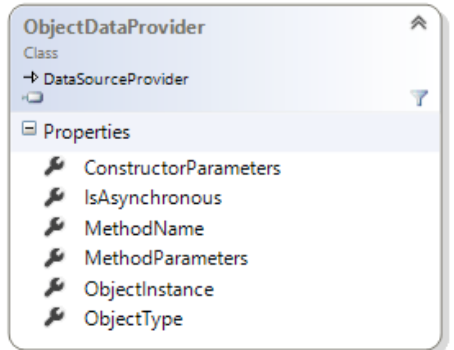
\includegraphics[scale=0.35]{ObjectDataProvider.png}

\begin{lstlisting}[language=xml]
<Window.Resources>
    <ObjectDataProvider x:Key="Alignments"
        MethodName="GetNames"
        ObjectType="{x:Type sys:Enum}">
    <ObjectDataProvider.MethodParameters>
        <x:Type TypeName="VerticalAlignment" />
    </ObjectDataProvider.MethodParameters>
    </ObjectDataProvider>
</Window.Resources>

<!-- Verwendung -->
<ComboBox ItemsSource="{Binding Source={StaticResource Alignments}}" />
\end{lstlisting}
\paragraph{DataBinding Debuggen} Man hat diverse Möglichkeiten die Abläufe hinter dem DataBinding sichtbar zu machen.
\begin{enumerate}
\item Direkt im Binding konfigurieren
\begin{lstlisting}[language=xml]
<!-- System.Diagnostics-Namespace - hinzufuegen -->
xmlns:diag="clr-namespace:System.Diagnostics;assembly=WindowsBase"
<!-- Binding Ausdruck um Setzten des TraceLevels erweitern -->
<TextBlock Text="{Binding ElementName=stack, Path=InvalidPath, diag:PresentationTraceSources.TraceLevel=High}" />
\end{lstlisting}
\item Dummy Converter schreiben
\begin{lstlisting}
public class DebugDummyConverter : IValueConverter
{
    public object Convert(object value, Type targetType, object parameter, CultureInfo culture)
    {
        return value;
    }
    public object ConvertBack(object value, Type targetType, object parameter, CultureInfo culture)
    {
        return value;
    }
}
\end{lstlisting}
\begin{lstlisting}[language=xml]
<Window.Resources> ... <local:DebugDummyConverter x:Key="MyDummy" /> ... </Window.Resources>
...
<TextBlock Text="{Binding ElementName=stack, Path=InvalidPath, Converter={StaticResource MyDummy}}" />
\end{lstlisting}
\item In VisualStudio DataBinding Debugging auf "{}All"{} setzten und im Output-Window nach \verb+Syste.Windows.Data+ suchen.
\end{enumerate}

\subsection{INotifyPropertyChanged (INPC)}
\begin{itemize}
    \item Benötigt bei: \code{OneWay}, \code{TwoWay}
    \item Nicht benötigt bei: \code{OneTime}, \code{OneWayToSource}
\end{itemize}




